\section{Mechanical Model of a Quantum Field}

To build intuition for quantum fields, it is useful to begin with a simple mechanical system: a chain of coupled elastic strings. This model arises as the \textit{continuum limit} of a one-dimensional lattice of \(N\) atoms, and already captures many of the essential features of field theories.

We consider a \textbf{meta-stable} system, meaning that its configuration does not change drastically under the action of a small perturbing force.\footnote{In fact, every physical system is meta-stable in this sense: if a small perturbation could radically alter its configuration, it could not persist in a stable state.} Thus, there must exist a restoring force that drives the system back toward equilibrium.

For a small displacement \(y\) from equilibrium, the restoring force can be expanded in a Taylor series:
\[
    F(y) = F(0) + \left.\frac{dF}{dy}\right|_{y=0} y + \dots
    = -|\kappa|\, y + \mathcal{O}(y^2),
\]
where we set \(F(0) = 0\) (no force at equilibrium) and require \(\left.\tfrac{dF}{dy}\right|_{y=0} = -|\kappa| < 0\) (restoring behavior). The linear term dominates for sufficiently small displacements, showing that any meta-stable system can be modeled, to first approximation, as a collection of coupled harmonic oscillators.

The simplest realization is a chain of \(N\) identical atoms, each of mass \(m\), connected by springs with spring constant \(\kappa\) and arranged along a line with equilibrium spacing \(\Delta\). The total length of the chain is
\[
    L = N \Delta.
\]
The displacement of the \(i\)-th atom from its equilibrium position will be denoted by \(y_i(t)\). For simplicity, we restrict ourselves to transverse displacements along the \(y\)-axis, keeping the equilibrium positions along the \(x\)-axis fixed.

\begin{figure}[H]
    \begin{minipage}{0.45\textwidth}
        \centering
        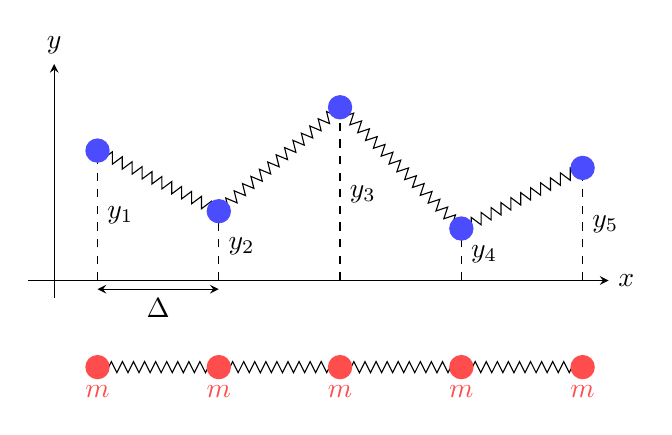
\begin{tikzpicture}[scale=1.1,>=stealth]

            % Horizontal spacing between masses
            \def\Deltax{1.4}

            % Random vertical positions (displacements)
            \def\yA{0.5}
            \def\yB{-0.2}
            \def\yC{1.0}
            \def\yD{-0.4}
            \def\yE{0.3}

            % Reference axes
            \draw[->] (-0.5,-1.2) -- (-0.5,1.5) node[anchor=south]{$y$};
            \draw[->] (-0.8,-1.0) -- (5*\Deltax-1.1,-1.0) node[anchor=west]{$x$};

            % --- Upper part: masses at different y ---
            % Mass vertical positions
            \coordinate (m1) at (0,\yA);
            \coordinate (m2) at (\Deltax,\yB);
            \coordinate (m3) at (2*\Deltax,\yC);
            \coordinate (m4) at (3*\Deltax,\yD);
            \coordinate (m5) at (4*\Deltax,\yE);

            % Springs (zigzag lines)
            \draw[decorate,decoration={zigzag,segment length=4pt,amplitude=2pt}] (m1) -- (m2);
            \draw[decorate,decoration={zigzag,segment length=4pt,amplitude=2pt}] (m2) -- (m3);
            \draw[decorate,decoration={zigzag,segment length=4pt,amplitude=2pt}] (m3) -- (m4);
            \draw[decorate,decoration={zigzag,segment length=4pt,amplitude=2pt}] (m4) -- (m5);

            % Segments and spacings
            \foreach \i/\y in {1/\yA, 2/\yB, 3/\yC, 4/\yD, 5/\yE} {
                    \draw[dashed] (\i*\Deltax-\Deltax,-1) -- (\i*\Deltax-\Deltax,\y) node[midway,right] {$y_{\i}$};
                }
            \draw[<->] (0,-1.1) -- (\Deltax,-1.1) node[midway,below] {$\Delta$};

            % Masses (blue circles)
            \foreach \m in {m1,m2,m3,m4,m5}{
                    \fill[blue!70] (\m) circle (4pt);
                }

            % --- Lower part: horizontal chain ---
            \begin{scope}[yshift=-2cm]
                % Horizontal positions
                \coordinate (n1) at (0,0);
                \coordinate (n2) at (\Deltax,0);
                \coordinate (n3) at (2*\Deltax,0);
                \coordinate (n4) at (3*\Deltax,0);
                \coordinate (n5) at (4*\Deltax,0);

                % Springs
                \draw[decorate,decoration={zigzag,segment length=4pt,amplitude=2pt}] (n1) -- (n2);
                \draw[decorate,decoration={zigzag,segment length=4pt,amplitude=2pt}] (n2) -- (n3);
                \draw[decorate,decoration={zigzag,segment length=4pt,amplitude=2pt}] (n3) -- (n4);
                \draw[decorate,decoration={zigzag,segment length=4pt,amplitude=2pt}] (n4) -- (n5);

                % Masses (red circles)
                \foreach \n in {n1,n2,n3,n4,n5}{
                        \fill[red!70] (\n) circle (4pt);
                        \node[red!70,below=3pt] at (\n) {$m$};
                    }
            \end{scope}

        \end{tikzpicture}
    \end{minipage}
    \hfill
    \begin{minipage}{0.45\textwidth}
        \(y_i=0\) is the equilibrium position of the \(i\)-th atom. The springs exert restoring forces proportional to the relative displacements of neighboring atoms: each atom is under the influence of the neighboring springs, describing a local interaction.

        \(y_i\neq0\) describes the small oscillations around the equilibrium position: transverse \textbf{excitations} of the lattice.
    \end{minipage}
\end{figure}

In the limit \(N\to\infty\) and \(\Delta \to 0\) with \(L\) fixed, the discrete index \(i\) becomes a continuous spatial coordinate and the displacements \(y_i(t)\) become a continuous field \(\phi(x,t)\). This \textbf{continuum limit} transforms the system of coupled oscillators into a continuous field, allowing us to understand the dynamics of fields in terms of familiar mechanical concepts.

\subsection{Discrete case}

To study the dynamics of the chain we employ the Euler--Lagrange equations.
The Lagrangian of the system is constructed as the difference between the kinetic and potential energy contributions of each atom:
\[
    \begin{aligned}
        L & = \sum_{j=1}^N \left[ \frac{1}{2} m \dot{y}_j^2 - \frac{1}{2} k \left(y_j - y_{j+1}\right)^2 \right]                      \\
          & = \sum_{j=1}^N \left[ \frac{1}{2} m \dot{y}_j^2 - \frac{1}{2} \kappa \left(\frac{y_j - y_{j+1}}{\Delta}\right)^2 \right],
    \end{aligned}
\]
where we impose periodic boundary conditions \(j \to j+N\)\footnote{In other words, the first and the last atoms in the chain interact with each other.} and we renamed the spring constant \(k\) as \(\kappa = k \Delta^2\), which is now more of a \textit{coupling constant} between neighboring atoms.

We are assuming small oscillations around the equilibrium configuration, such that the relative displacement between neighboring atoms is small compared to the natural lattice spacing \(\Delta\):
\[
    \frac{y_j - y_{j+1}}{\Delta} \ll 1.
\]

It is worth noting that the coupling constant \(\kappa\) has the dimension of an energy, and can be written as
\[
    \kappa = m v^2,
\]
where \(v\) is a characteristic velocity associated with the propagation of disturbances along the chain. With this identification, the Lagrangian becomes
\[
    L = \frac{1}{2}m \sum_{j=1}^{N} \left[ \dot{y}_j^2(t)
        - v^2\left(\frac{y_j - y_{j+1}}{\Delta}\right)^2  \right],
\]
where the first term corresponds to the kinetic energy of the atoms, while the second encodes the elastic potential energy due to the coupling between neighbors.

The time evolution of the system is obtained by applying the principle of least action:
the motion is such that the variation of the action vanishes,
\[
    S = \int L \, \mathrm{d}t, \qquad \delta S = 0,
\]
which leads to the Euler--Lagrange equations governing the dynamics of the chain.
Recalling the general form
\[
    \frac{\mathrm{d}}{\mathrm{d} t} \frac{\partial L}{\partial \dot{y}_j}
    = \frac{\partial L}{\partial {y}_j},
    \qquad j = 1, \dots , N,
\]
we obtain the governing equations of motion:
\[
    \ddot{y}_j (t)
    = -\,v^2 \left(\frac{2y_j - y_{j+1} - y_{j-1}}{\Delta^2}\right).
\]
This result clearly describes a system of coupled harmonic oscillators: the displacement of the \(j\)-th atom is influenced not only by its own position but also by the relative positions of its nearest neighbors, \((j+1)\) and \((j-1)\).
In other words, each atom is bound to oscillate around equilibrium under the restoring force arising from the springs that connect it to its neighbors.

Solving such a system directly is not convenient, since the equations are not independent. However, there is a natural way to simplify the problem by exploiting the translational symmetry of the lattice. The key idea is to perform a \textit{discrete Fourier transform} of the displacements, which allows us to rewrite the dynamics in terms of normal modes of oscillation. Since \(y_j(t)\) has to be periodic (\(y_j(t) = y_{j+N}(t)\)), we can write:
\[
    y_j(t) = \frac{1}{\sqrt{N}} \sum_{\sigma=1}^{N} e^{i\frac{2\pi}{N}\sigma j} \tilde{y}_{\sigma}(t).
\]
In this new representation, each mode corresponds to a collective oscillation of the entire chain with a definite wavelength. From a mathematical perspective, this amounts to diagonalizing the interaction matrix: the coupling between neighbors is replaced by a set of independent equations for the Fourier modes. In physical terms, the Fourier transform identifies the proper "coordinates" in which the energy of the system can be expressed as a sum of independent contributions, one for each mode.\footnote{In other words, instead of tracking the motion of individual atoms, which are strongly coupled, we describe the system in terms of delocalized excitations (the normal modes), each evolving independently. This step paves the way to the field interpretation: in the continuum limit, these modes will be interpreted as excitations of a quantum field.}

Now, by substituting in the equation of motion, we can decouple the system:
\[
    \begin{aligned}
        \frac{1}{\sqrt{N}} \sum_{\sigma=1}^{N} e^{i\frac{2\pi}{N}\sigma j} \ddot{\tilde{y}}_{\sigma} & = \frac{-1}{\sqrt{N}} \left(\frac{v}{\Delta}\right)^2 \left[ 2 \sum_{\sigma=1}^{N} e^{i\frac{2\pi}{N}\sigma j} \tilde{y}_{\sigma} - \sum_{\sigma=1}^{N} e^{i\frac{2\pi}{N}\sigma (j-1)} \tilde{y}_{\sigma} - \sum_{\sigma=1}^{N} e^{i\frac{2\pi}{N}\sigma (j+1)} \tilde{y}_{\sigma}\right] \\
                                                                                                     & = \frac{-1}{\sqrt{N}} \left(\frac{v}{\Delta}\right)^2 \sum_{\sigma=1}^{N} e^{i\frac{2\pi}{N}\sigma j} \tilde{y}_{\sigma} \left[ 2 - e^{-i\frac{2\pi}{N}\sigma} - e^{i\frac{2\pi}{N}\sigma}\right]                                                                                          \\
                                                                                                     & = \frac{-1}{\sqrt{N}} \left(\frac{v}{\Delta}\right)^2 \sum_{\sigma=1}^{N} e^{i\frac{2\pi}{N}\sigma j} \tilde{y}_{\sigma} \left[ 2 - 2 \cos(\frac{2\pi}{N}\sigma)\right]                                                                                                                    \\
        \iff \ddot{\tilde{y}}_{\sigma}(t)                                                            & = - 2 \frac{v^2}{\Delta^2} \left[ 1 - \cos(\frac{2\pi}{N}\sigma)\right] \tilde{y}_{\sigma}(t) = - \left( \frac{2v}{\Delta} \sin(\frac{\pi\sigma}{N}) \right)^2 \tilde{y}_{\sigma}(t),
    \end{aligned}
\]
where we have made use of the trigonometric identity
\((1 - \cos(2\theta)) = 2\sin^2(\theta)\). This leads to the following set of equations for the Fourier modes:
\[
    \begin{aligned}
        \ddot{\tilde{y}}_{\sigma}(t) & = - \omega^2_{\sigma}\, \tilde{y}_{\sigma}(t),
        \quad                        &                                                                & \forall \, \sigma = 1,2,\dots,N, \\
        \omega_{\sigma}              & = \frac{2v}{\Delta} \, \sin\!\left(\frac{\pi\sigma}{N}\right).
    \end{aligned}
\]
%
Each Fourier component \(\tilde{y}_{\sigma}(t)\) evolves independently and satisfies the equation of a simple harmonic oscillator with characteristic frequency \(\omega_{\sigma}\).
In other words, the original coupled system of atoms has been diagonalized into a set of \(N\) decoupled oscillators, each associated with a normal mode of vibration.

The general solution for each mode is therefore given by a linear combination of oscillatory functions:
\[
    \tilde{y}_{\sigma}(t)
    = A_{\sigma} e^{-i \omega_{\sigma} t} + B_{\sigma} e^{+i \omega_{\sigma} t},
\]
where the constants \(A_{\sigma}\) and \(B_{\sigma}\) are determined by the initial conditions.
Physically, these modes correspond to standing waves propagating through the chain, each characterized by a discrete wave number and its corresponding frequency.

In practice, we will keep only the negative exponential,
\[
    \tilde{y}_{\sigma}(t) = A_{\sigma} e^{-i \omega_{\sigma} t},
\]
since the positive-frequency solution is automatically recovered as the complex conjugate.
This choice avoids redundancy and is particularly convenient when later quantizing the system, because creation and annihilation operators will naturally emerge from the decomposition into \(e^{-i\omega t}\) and its conjugate.

Now we can plug the solution for the Fourier modes back into the inverse transform in order to recover the displacement of the \(j\)-th atom:
\[
    \begin{aligned}
        y_j(t) & = \frac{1}{\sqrt{N}} \sum_{\sigma=1}^{N} e^{i\frac{2\pi}{N}\sigma j} \tilde{y}_{\sigma}(t)                                                   \\
               & = \frac{1}{\sqrt{N}} \sum_{\sigma=1}^{N} A_{\sigma} e^{i \left( \frac{2\pi}{N}\sigma j - \omega_{\sigma} t \right)}                          \\
               & = \frac{1}{\sqrt{N}} \sum_{\sigma=1}^{N} A_{\sigma} e^{i \left( \frac{2\pi}{N}\frac{\sigma}{\Delta} (\Delta j) - \omega_{\sigma} t \right)},
    \end{aligned}
\]
Here we have reintroduced the lattice spacing \(\Delta\), so that the quantity \(\Delta j\) corresponds exactly to the physical position \(x\) of the \(j\)-th atom along the chain.

This expression shows that the displacement of each atom can be written as a linear superposition of plane waves (like \textit{sound waves}). In particular, the system supports \(N\) different wave numbers, each corresponding to one Fourier mode:
\[
    \kappa_{\sigma} = \frac{2\pi}{N} \frac{\sigma}{\Delta} = \frac{2\pi}{\lambda_{\sigma}}, \qquad \sigma = 1,2,\dots,N,
\]
with associated discrete wavelengths
\[
    \lambda_{\sigma} = \frac{N\Delta}{\sigma} = N\Delta, \, \frac{N\Delta}{2}, \dots, \Delta.
\]

\begin{remark}
    The propagation speed of each mode is obtained as the ratio between its frequency and its wave number:
    \[
        v_{\sigma} = \frac{\omega_{\sigma}}{\kappa_{\sigma}}
        = \frac{\tfrac{2v}{\Delta}\,\sin\!\left(\tfrac{\pi\sigma}{N}\right)}{\tfrac{2\pi}{N}\tfrac{\sigma}{\Delta}}
        = v \,\frac{N}{\pi\sigma} \,\sin\!\left(\tfrac{\pi\sigma}{N}\right).
    \]
    Introducing the parameter \(\theta_{\sigma} = \tfrac{\pi\sigma}{N}\), this can be written in the compact form
    \[
        v_{\sigma} = v\,\frac{\sin(\theta_{\sigma})}{\theta_{\sigma}}.
    \]
    This result shows that each Fourier mode propagates with a distinct phase velocity, depending on the ratio \(\sigma/N\).
    In the continuum limit \(N \to \infty\) with \(\sigma/N \to 0\), one has \(\theta_{\sigma} \to 0\) and therefore
    \[
        \lim_{\theta_{\sigma}\to 0} \frac{\sin(\theta_{\sigma})}{\theta_{\sigma}} = 1,
    \]
    so all modes propagate with the same velocity \(v_{\sigma} \sim v\). This recovers the expected propagation speed of sound waves in the continuous chain.
\end{remark}

\begin{remark}
    The actual number of independent vibrational degrees of freedom is \(N-1\), since the \(N\)-th mode corresponds to a zero frequency:
    \[
        \omega_{\sigma=N} = \frac{2v}{\Delta}\,\sin\!\left(\pi \frac{N}{N}\right) = 0.
    \]
    This means that \(\tilde{y}_N(t)\) does not oscillate in time. Physically, this mode represents a uniform translation of the entire chain, where all atoms are displaced by the same amount. As such, it does not contribute to the internal vibrational dynamics, and the only genuine oscillatory modes are the first \(N-1\).
\end{remark}

\begin{figure}[H]
    \begin{minipage}{0.5\textwidth}
        Moreover we can show that the waves with \(\sigma = s\) and \(\sigma = N-s\) in general have the same frequency \(\omega_s\), since:
        \[
            \begin{aligned}
                \omega_{N-s} & = \frac{2v}{\Delta}\,\sin\!\left(\pi \frac{N-s}{N}\right)           \\
                             & = \frac{2v}{\Delta}\,\sin\!\left(\pi -\frac{\pi s}{N}\right)        \\
                             & = \frac{2v}{\Delta}\,\sin\!\left(\frac{\pi s}{N}\right) = \omega_s.
            \end{aligned}
        \]
    \end{minipage}
    \hfill
    \begin{minipage}{0.45\textwidth}
        \centering
        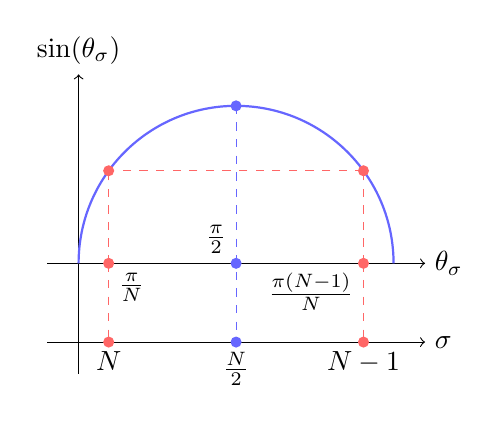
\begin{tikzpicture}[scale=2]
            \draw[->] (-0.2,0) -- (2.2,0) node[right] {$\theta_{\sigma}$};
            \draw[->] (-0.2,-0.5) -- (2.2,-0.5) node[right] {$\sigma$};
            \draw[->] (0,-0.7) -- (0,1.2) node[above] {$\sin(\theta_{\sigma})$};

            \draw[thick, blue!60] (0,0) arc[start angle=180,end angle=0,radius=1];

            \def\N{5}
            \def\xone{pi/\N}
            \def\xtwo{pi*(\N-1)/\N}

            \coordinate (A) at ({1+cos(180*\xone/pi)},{sin(180*\xone/pi)});
            \coordinate (B) at ({1+cos(180*\xtwo/pi)},{sin(180*\xtwo/pi)});
            \coordinate (-A) at ({1+cos(180*\xone/pi)},-0.5);
            \coordinate (-B) at ({1+cos(180*\xtwo/pi)},-0.5);

            \draw[dashed, red!60] (A|-0,0) -- (A);
            \draw[dashed, red!60] (B|-0,0) -- (B);
            \draw[dashed, red!60] (A|-0,0) -- (-A);
            \draw[dashed, red!60] (B|-0,0) -- (-B);
            \draw[dashed, red!60] (A) -- (B);
            \draw[dashed, blue!60] (1,1) -- (1,-0.5);

            \node[below left] at (A|-0,0) {$\frac{\pi(N-1)}{N}$};
            \node[below right] at (B|-0,0) {$\frac{\pi}{N}$};
            \node[below] at (A|-0,-0.5) {$N-1$};
            \node[below] at (B|-0,-0.5) {$N$};
            \node[above left] at (1,0) {$\frac{\pi}{2}$};
            \node[below] at (1,-0.5) {$\frac{N}{2}$};

            \fill[red!60] (A) circle (1pt);
            \fill[red!60] (B) circle (1pt);
            \fill[red!60] (A|-0,0) circle (1pt);
            \fill[red!60] (B|-0,0) circle (1pt);
            \fill[red!60] (A|-0,-0.5) circle (1pt);
            \fill[red!60] (B|-0,-0.5) circle (1pt);
            \fill[blue!60] (1,0) circle (1pt);
            \fill[blue!60] (1,1) circle (1pt);
            \fill[blue!60] (1,-0.5) circle (1pt);
        \end{tikzpicture}
    \end{minipage}
\end{figure}

We can interpret the two modes with the same frequency as forming a single complex degree of freedom. This interpretation is supported by the observation that the original variable \(y_j\) is real, even though it is expressed as a sum of complex exponentials:
\[
    \begin{aligned}
        y_j(t)   & = \frac{1}{\sqrt{N}} \sum_{\sigma=1}^{N} e^{i\frac{2\pi}{N}\sigma j} \tilde{y}_{\sigma}(t),    \\
        y_j^*(t) & = \frac{1}{\sqrt{N}} \sum_{\sigma=1}^{N} e^{-i\frac{2\pi}{N}\sigma j} \tilde{y}_{\sigma}^*(t). \\
    \end{aligned}
\]
Thus, by requiring that the two expressions coincide, we can compute:
\[
    \begin{aligned}
        \sum_{\sigma=1}^{N} e^{i\frac{2\pi}{N}\sigma j} \tilde{y}_{\sigma}(t)                  & = \sum_{\sigma=1}^{N} e^{-i\frac{2\pi}{N}\sigma j} \tilde{y}_{\sigma}^*(t), \\
        \sum_{\sigma=N-1}^{0} e^{i\frac{2\pi}{N}(N-\sigma) j} \tilde{y}_{N-\sigma}(t)          & = \sum_{\sigma=1}^{N} e^{-i\frac{2\pi}{N}\sigma j} \tilde{y}_{\sigma}^*(t), \\
        \sum_{\sigma=N-1}^{0} e^{i2\pi j} e^{-i\frac{2\pi}{N}\sigma j} \tilde{y}_{N-\sigma}(t) & = \sum_{\sigma=1}^{N} e^{-i\frac{2\pi}{N}\sigma j} \tilde{y}_{\sigma}^*(t), \\
        \sum_{\sigma=N-1}^{0} e^{-i\frac{2\pi}{N}\sigma j} \tilde{y}_{N-\sigma}(t)             & = \sum_{\sigma=1}^{N} e^{-i\frac{2\pi}{N}\sigma j} \tilde{y}_{\sigma}^*(t), \\
        \sum_{\sigma=1}^{N} e^{-i\frac{2\pi}{N}\sigma j} \tilde{y}_{N-\sigma}(t)               & = \sum_{\sigma=1}^{N} e^{-i\frac{2\pi}{N}\sigma j} \tilde{y}_{\sigma}^*(t), \\
        \sum_{\sigma=1}^{N} \left[ \tilde{y}_{N-\sigma}(t) - \tilde{y}_{\sigma}^*(t) \right]   & = 0,
    \end{aligned}
\]
which lead us to conclude that \(\tilde{y}_{N-\sigma}(t) = \tilde{y}_{\sigma}^*(t)\).\footnote{In the first step, we rename the summation index on the right-hand side of the equation, replacing each \(\sigma\) with \(N - \sigma\). We then use the periodicity condition \(e^{i 2\pi j} = 1\) to simplify the exponential factor. Next, we reverse the order of summation and, since the terms corresponding to \(\sigma = 0\) and \(\sigma = N\) are identical, we can safely rewrite the sum over the range \(1 \leq \sigma \leq N\).}

Now we are in a position to compute the total number of independent vibrational degrees of freedom. To do so, we must distinguish two cases:
\begin{itemize}
    \item \textbf{If \(N\) is even (\(N = 2l\))}, the total number of pairs of harmonic oscillators with the same frequency (denoted by \(m\)) is
          \[
              m = \frac{2l - 2}{2} = l - 1 .
          \]
          In this case we have to exclude the modes \(\sigma = N\) and \(\sigma = \frac{N}{2}\). The reason is that, when \(N\) is even, the mode with index \(\sigma = \frac{N}{2}\) is self-conjugate, since it coincides with its complementary mode \(\sigma = N - \frac{N}{2} = \frac{N}{2}\).

    \item \textbf{If \(N\) is odd (\(N = 2l+1\))}, the total number of such oscillator pairs is
          \[
              m = \frac{(2l+1) - 1}{2} = l .
          \]
          Here the only index that must be removed is \(\sigma = N\), since \(\frac{N}{2}\) is not an integer and therefore does not correspond to any mode index.
\end{itemize}
The two oscillators associated with the same frequency can be regarded as components of a single complex degree of freedom. In this representation, the physical displacement corresponds to the real part of the complex variable, while the imaginary part encodes the redundant conjugate mode.

We can now exploit the solutions obtained in the new basis to diagonalize the Hamiltonian, since the transformation allows us to rewrite it in terms of independent normal modes, each of which behaves as an uncoupled harmonic oscillator. Let us temporarily neglect the contributions from the modes $\sigma = \frac{N}{2}, N$. Then the kinetic energy can be rewritten as
\[
    \begin{aligned}
        T & = \frac{1}{2}m \sum_{j=1}^N \dot{y}_j^2                                                                                                                                                                                                                                                                                                                                       \\
          & = \frac{1}{2}m \sum_{j=1}^N \frac{1}{N} \sum_{\sigma=1}^{\frac{N}{2}-1} \left( e^{i \frac{2\pi}{N}\sigma j} \dot{\tilde{y}}_{\sigma} + e^{-i \frac{2\pi}{N}\sigma j} \dot{\tilde{y}}_{N-\sigma} \right) \sum_{\xi=1}^{\frac{N}{2}-1} \left( e^{i \frac{2\pi}{N}\xi j} \dot{\tilde{y}}_{\xi} + e^{-i \frac{2\pi}{N}\xi j} \dot{\tilde{y}}_{N-\xi} \right)                      \\
          & = \frac{1}{2}m \sum_{\sigma,\xi=1}^{\frac{N}{2}-1} \left[ \dot{\tilde{y}}_{\sigma} \dot{\tilde{y}}_{\xi} \left( \frac{1}{N} \sum_{j=1}^N e^{i \frac{2\pi}{N}(\sigma+\xi) j} \right) + \dot{\tilde{y}}_{N-\sigma} \dot{\tilde{y}}_{\xi} \left( \frac{1}{N} \sum_{j=1}^N e^{i \frac{2\pi}{N}(\xi-\sigma) j} \right) \right.                                                     \\
          & \qquad\qquad\qquad+ \left. \dot{\tilde{y}}_{\sigma} \dot{\tilde{y}}_{N-\xi} \left( \frac{1}{N} \sum_{j=1}^N e^{i \frac{2\pi}{N}(\sigma-\xi) j} \right) + \dot{\tilde{y}}_{N-\sigma} \dot{\tilde{y}}_{N-\xi} \left( \frac{1}{N} \sum_{j=1}^N e^{-i \frac{2\pi}{N}(\sigma+\xi) j} \right) \right]                                                                               \\
          & = \frac{1}{2}m \sum_{\sigma,\xi=1}^{\frac{N}{2}-1} \left( \dot{\tilde{y}}_{\sigma} \dot{\tilde{y}}_{\xi} \, \delta_{\sigma+\xi, 0} + \dot{\tilde{y}}_{N-\sigma} \dot{\tilde{y}}_{\xi} \, \delta_{\sigma,\xi} + \dot{\tilde{y}}_{\sigma} \dot{\tilde{y}}_{N-\xi} \, \delta_{\sigma,\xi} + \dot{\tilde{y}}_{N-\sigma} \dot{\tilde{y}}_{N-\xi} \, \delta_{\sigma+\xi, 0} \right) \\
          & = \frac{1}{2}m \sum_{\sigma=1}^{\frac{N}{2}-1} \left( 2 \dot{\tilde{y}}_{\sigma} \dot{\tilde{y}}_{N-\sigma} \right) = m \sum_{\sigma=1}^{\frac{N}{2}-1} \dot{\tilde{y}}_{\sigma} \dot{\tilde{y}}_{\sigma}^* = m \sum_{\sigma=1}^{\frac{N}{2}-1} \vert \dot{\tilde{y}}_{\sigma} \vert ^2.
    \end{aligned}
\]
The sum over $j$ enforce orthogonality, which manifests as Kronecker deltas. These deltas select only the diagonal terms, pairing each mode $\sigma$ with its complex conjugate $N-\sigma$. The final expression is a sum over independent Fourier modes, where the kinetic energy is simply the mass times the squared modulus of the time derivative of each mode amplitude. Now for the potential energy:
\[
    \begin{aligned}
        V & = \frac{1}{2} m \left( \frac{v}{\Delta} \right)^2 \sum_{j=1}^N \left( y_j - y_{j+1} \right)^2 =                                                                                                                                                                                                               \\
          & = \frac{1}{2} m \left( \frac{v}{\Delta} \right)^2 \sum_{j=1}^N \left[\sum_{\sigma=1}^{\frac{N}{2}-1} \left[ \left( e^{i \frac{2\pi}{N}\sigma j} \tilde{y}_{\sigma} + e^{-i \frac{2\pi}{N}\sigma j} \tilde{y}_{N-\sigma} \right) \right.\right.                                                                \\
          & \qquad\qquad\qquad\qquad \left.\left.- \left( e^{i \frac{2\pi}{N}\sigma (j+1)} \tilde{y}_{\sigma} + e^{-i \frac{2\pi}{N}\sigma (j+1)} \tilde{y}_{N-\sigma} \right) \right] \right]^2                                                                                                                          \\
          & = \frac{1}{2} m \left( \frac{v}{\Delta} \right)^2 \sum_{j=1}^N \left[\sum_{\sigma=1}^{\frac{N}{2}-1} \left[ \tilde{y}_{\sigma} e^{i \alpha_{\sigma}  j} \left( 1 - e^{i \alpha_{\sigma}} \right) + \tilde{y}_{N-\sigma} e^{-i \alpha_{\sigma}  j} \left( 1 - e^{-i \alpha_{\sigma}} \right) \right] \right]^2 \\
          & = \frac{1}{2} m \left( \frac{v}{\Delta} \right)^2 \sum_{j=1}^N \left[\sum_{\sigma=1}^{\frac{N}{2}-1} 2i \sin(\frac{\alpha_{\sigma}}{2}) \left( - \tilde{y}_{\sigma} e^{i \alpha_{\sigma} (j+\tfrac12)} + \tilde{y}_{N-\sigma} e^{-i \alpha_{\sigma} (j+\tfrac12)} \right) \right]^2,
    \end{aligned}
\]
where \(\alpha_{\sigma} = \frac{2\pi}{N}\sigma\). Now, using again the sum over \(j\) to enforce orthogonality (noting that the term \(j+\tfrac12\) on the exponential does not influence the result since it is canceled in cross-terms, while diagonal terms are zeroed by \(\delta_{\sigma+\xi,0}\)) and recalling the expression for \(\omega_{\sigma}\), we arrive to the diagonal form of the potential:
\[
    V = \frac{1}{2} m \left( \frac{v}{\Delta} \right)^2 \sum_{\sigma=1}^{\frac{N}{2}-1} 8 \sin(\frac{\alpha_{\sigma}}{2})^2 \tilde{y}_{\sigma}\tilde{y}_{N-\sigma} = m \sum_{\sigma=1}^{\frac{N}{2}-1} \omega_{\sigma}^2 \vert \tilde{y}_{\sigma} \vert^2.
\]
Finally, by adding the contributions from the modes $\sigma = \frac{N}{2}, N$, we arrive to the diagonal form of our Lagrangian:
\[
    L = m \sum_{\sigma=1}^{\frac{N}{2}-1} \left( \vert \dot{\tilde{y}}_{\sigma} \vert ^2 - \omega_{\sigma}^2 \vert \tilde{y}_{\sigma} \vert^2 \right) + \frac{m}{2} \left( \dot{\tilde{y}}_{\frac{N}{2}}^2 + \dot{\tilde{y}}_{N}^2 - \omega_{\frac{N}{2}}^2 \tilde{y}_{\frac{N}{2}}^2 \right),
\]
since \(\omega_N = 0\).\footnote{Let us remember that the \(\frac{N}{2}\)-th mode is absent when \(N\) is odd.} Thus, in the end, we have \(\tfrac{N-2}{2}\) complex degrees of freedom from the first term, which become \(N-2\) real degrees of freedom with \(\tfrac{N-2}{2}\) different frequencies, while the second term contributes with 2 real degrees of freedom.

In practice, the diagonalization procedure eliminates the cross-terms that mix different coordinates, leaving a sum of quadratic contributions that can be interpreted as the energies of the individual modes. As a result, the system is reduced to a collection of independent harmonic oscillators, each characterized by its own frequency.

\subsubsection{Quantization}

In order to proceed with the quantization of the system, it is useful to briefly recall the main ingredients of the quantum harmonic oscillator.

We start from the Hamiltonian operator expressed in terms of the position and momentum operators \(\hat y\) and \(\hat p\):
\[
    \hat{H} = \frac{\hat{p}^2}{2m} + \frac{1}{2} m \omega^2 \hat{y}^2 .
\]

The canonical quantization rule imposes the commutation relation between \(\hat y\) and \(\hat p\):
\[
    [\hat{y}, \hat{p}] = i \hbar .
\]
It is then convenient to introduce the so--called ladder (or creation/annihilation) operators:
\[
    \hat{a} = \sqrt{\frac{m\omega}{2\hbar}} \, \hat{y} + \frac{i}{\sqrt{2m\hbar\omega}} \, \hat{p},
    \qquad
    \hat{a}^\dagger = \sqrt{\frac{m\omega}{2\hbar}} \, \hat{y} - \frac{i}{\sqrt{2m\hbar\omega}} \, \hat{p}.
\]
These operators satisfy the commutation relation \( [\hat{a}, \hat{a}^\dagger] = 1 \). In terms of \(\hat{a}\) and \(\hat{a}^\dagger\), the Hamiltonian takes the following simple form:
\[
    \hat{H} = \hbar \omega \left(\hat{a}^\dagger \hat{a} + \tfrac{1}{2}\right).
\]
Finally, the position and momentum operators can be expressed back in terms of the ladder operators as
\[
    \hat{y} = \sqrt{\frac{\hbar}{2m\omega}} \, \big(\hat{a} + \hat{a}^\dagger \big),
    \qquad
    \hat{p} = i \sqrt{\frac{m\hbar\omega}{2}} \, \big(\hat{a}^\dagger - \hat{a}\big).
\]
We now examine the action of the ladder operators by considering their commutators with the Hamiltonian. To understand how the operators affect the energy states, let us compute the commutator with the annihilation operator $\hat a$:
\[
    [\hat H, \hat a] = \hbar \omega \, [\hat a^\dagger \hat a, \hat a].
\]
Using the general identity $[AB,C] = A[B,C] + [A,C]B$, we obtain
\[
    [\hat a^\dagger \hat a, \hat a] = \hat a^\dagger [\hat a,\hat a] + [\hat a^\dagger, \hat a] \hat a = -\hat a,
\]
so that
\[
    [\hat H, \hat a] = - \hbar \omega \, \hat a.
\]
Similarly, for the creation operator $\hat a^\dagger$, we have
\[
    [\hat H, \hat a^\dagger] = \hbar \omega \, [\hat a^\dagger \hat a, \hat a^\dagger] = \hbar \omega \, \hat a^\dagger.
\]

From these commutators, one can immediately deduce the action of the Hamiltonian on the states $\hat a |n\rangle$ and $\hat a^\dagger |n\rangle$. Using $\hat H |n\rangle = \hbar \omega \left(n + \tfrac12\right) |n\rangle$, we find
\[
    \hat H (\hat a |n\rangle) = (\hat a \hat H + [\hat H, \hat a]) |n\rangle = \hbar \omega \left(n - \tfrac12\right) (\hat a |n\rangle),
\]
\[
    \hat H (\hat a^\dagger |n\rangle) = (\hat a^\dagger \hat H + [\hat H, \hat a^\dagger]) |n\rangle = \hbar \omega \left(n + \tfrac32\right) (\hat a^\dagger |n\rangle).
\]
These results show explicitly that $\hat a$ lowers the energy of a state by one quantum $\hbar \omega$, while $\hat a^\dagger$ raises the energy by the same amount.

It is convenient to introduce the number operator, defined as
\[
    \hat N = \hat a^\dagger \hat a.
\]
This operator counts the number of quanta in a given state, since its action on the energy eigenstates is
\[
    \hat N |n\rangle = n |n\rangle.
\]
The ladder operators then have a simple interpretation in terms of the number operator: the annihilation operator $\hat a$ lowers the quantum number by one,
\[
    \hat a |n\rangle = \sqrt{n}\, |n-1\rangle,
\]
while the creation operator $\hat a^\dagger$ raises it by one,
\[
    \hat a^\dagger |n\rangle = \sqrt{n+1}\, |n+1\rangle.
\]
In this way, the states $|n\rangle$ can be constructed by successive application of $\hat a^\dagger$ starting from the vacuum state $|0\rangle$, and the number operator provides a direct measure of the excitation level of each state. These operators are the cornerstone for describing the spectrum and dynamics of the quantum harmonic oscillator.

We are now ready to quantize our \textit{mechanical string} with Lagrangian:
\[
    L = m \sum_{\sigma=1}^{\frac{N}{2}-1} \left( \vert \dot{\tilde{y}}_{\sigma} \vert ^2 + \omega_{\sigma}^2 \vert \tilde{y}_{\sigma} \vert^2 \right) + \frac{m}{2} \left( \dot{\tilde{y}}_{\frac{N}{2}}^2 + \dot{\tilde{y}}_{N}^2 + \omega_{\frac{N}{2}}^2 \tilde{y}_{\frac{N}{2}}^2 \right),
\]
It is useful to stress that each complex mode can be decomposed into its real and imaginary parts. In particular,
\[
    \tilde{y}_{\sigma} = \frac{1}{\sqrt{2}}(\Re \tilde{y}_{\sigma} + \Im \tilde{y}_{\sigma}) = \frac{\tilde{y}_{\sigma}^{(\mathrm{R})}+\tilde{y}_{\sigma}^{(\mathrm{I})}}{\sqrt{2}},
\]
so that the kinetic term can be written as
\[
    \vert \dot{\tilde{y}}_{\sigma} \vert ^2 = \frac{1}{2}\left[ (\dot{\tilde{y}}_{\sigma}^{(\mathrm{R})})^2 + (\dot{\tilde{y}}_{\sigma}^{(\mathrm{I})})^2 \right].
\]
For the real normal modes (e.g. the special indices \(\sigma=\frac{N}{2},N\)) we introduce the usual ladder operators \(\hat a_r,\hat a_r^\dagger\) and have
\[
    \hat{\tilde{y}}_{\sigma}^{(\mathrm{R})} = \sqrt{\frac{\hbar}{2 m \omega_{\sigma}}}\;(\hat a_{\sigma}^{(\mathrm{R})} + \hat a_{\sigma}^{\dagger(\mathrm{R})}),
    \qquad
    \hat{p}_{\sigma}^{(\mathrm{R})} = i\sqrt{\frac{m\hbar\omega_{\sigma}}{2}}\;(\hat a_{\sigma}^{(\mathrm{R})} - \hat a_{\sigma}^{\dagger(\mathrm{R})}),
\]
\[
    \hat{\tilde{y}}_{\sigma}^{(\mathrm{I})} = \sqrt{\frac{\hbar}{2 m \omega_{\sigma}}}\;(\hat a_{\sigma}^{(\mathrm{I})} + \hat a_{\sigma}^{\dagger(\mathrm{I})}),
    \qquad
    \hat{p}_{\sigma}^{(\mathrm{I})} = i\sqrt{\frac{m\hbar\omega_{\sigma}}{2}}\;(\hat a_{\sigma}^{(\mathrm{I})} - \hat a_{\sigma}^{\dagger(\mathrm{I})}),
\]
\[
    \hat{\tilde{y}}_{\frac{N}{2}} = \sqrt{\frac{\hbar}{2 m \omega_{\frac{N}{2}}}}\;(\hat a_{\frac{N}{2}} + \hat a_{\frac{N}{2}}^{\dagger}),
    \qquad
    \hat{p}_{\frac{N}{2}} = i\sqrt{\frac{m\hbar\omega_{\frac{N}{2}}}{2}}\;(\hat a_{\frac{N}{2}} - \hat a_{\frac{N}{2}}^{\dagger}),
\]

The natural framework to describe our quantized mechanical string is the \textbf{Fock space}, which allows us to account for an arbitrary number of excitations in each mode.

Formally, the Fock space is constructed as the direct sum of $n$-particle Hilbert spaces:
\[
    \mathcal{F} = \bigoplus_{n=0}^{\infty} \mathcal{H}^{(n)}
    = \mathcal{H}^{(0)} \oplus \mathcal{H}^{(1)} \oplus \mathcal{H}^{(2)} \oplus \dots,
\]
where $\mathcal{H}^{(0)} \cong \mathbb{C}$ represents the vacuum (the state with no phonons), while for $n \ge 1$ we define
\[
    \mathcal{H}^{(n)} = \underbrace{\mathcal{H}^{(1)} \otimes \mathcal{H}^{(1)} \otimes \dots \otimes \mathcal{H}^{(1)}}_{n \text{ times}}.
\]

Here, $\mathcal{H}^{(1)}$ is the Hilbert space of a single phonon, $\mathcal{H}^{(2)}$ is the space of two phonons, and in general $\mathcal{H}^{(n)}$ describes $n$ phonons. Each $\mathcal{H}^{(n)}$ is a subspace where the total number of excitations is fixed, and the tensor product structure reflects the fact that each phonon can occupy its own independent state within the mode basis.

The Fock space $\mathcal{F}$ as a whole thus contains all possible states with any number of phonons. This construction is crucial because in a quantum harmonic system the number of excitations is not fixed: the system can fluctuate between states with zero, one, or arbitrarily many phonons. Using the Fock space, we can systematically describe the action of creation and annihilation operators, build eigenstates of the total Hamiltonian, and keep track of the occupation numbers of all modes simultaneously.
\begin{itemize}
    \item \(\mathcal{H}^{(1)}\) is spanned by:
          \[
              \hat a_{\sigma}^{\dagger(\mathrm{R})} \ket{0}, \quad \hat a_{\sigma}^{\dagger(\mathrm{I})} \ket{0}, \quad \hat a_{\frac{N}{2}}^{\dagger} \ket{0}, \quad \sigma = 1, \dots, \frac{N}{2}-1,
          \]
          which we can denote more compactly as \(\hat a_{i}^{\dagger} \ket{0}\).
    \item \(\mathcal{H}^{(2)}\) is spanned by all two-phonon states, obtained by applying any two creation operators to the vacuum:
          \[
              \hat a_i^\dagger \hat a_j^\dagger \ket{0}, \qquad i,j = 1,2,\dots, N-1,
          \]
          including the possibility \(i=j\) (two phonons in the same mode).\footnote{One should properly symmetrize the two-phonon states, for instance:  \(\frac{1}{\sqrt{2}} \big( \hat a_i^\dagger \hat a_j^\dagger \ket{0} \pm \hat a_j^\dagger \hat a_i^\dagger \ket{0} \big)\), to ensure the correct bosonic/fermionic symmetry.}

    \item In general, \(\mathcal{H}^{(n)}\) is spanned by all $n$-phonon states:
          \[
              (\hat a_{i_1}^\dagger)^{n_1} (\hat a_{i_2}^\dagger)^{n_2} \dots (\hat a_{i_l}^\dagger)^{n_l} \ket{0}, \qquad \text{with } n_1 + n_2 + \dots + n_l = n,
          \]
          which include all possible distributions of $n$ phonons among the modes. Each \(\mathcal{H}^{(n)}\) is thus the subspace of the Fock space with exactly $n$ excitations.
\end{itemize}
Thus, we can define the vacuum more rigorously as
\[
    \ket{0} = \ket{0}_{\omega_1}^{(\mathrm{R})} \otimes \ket{0}_{\omega_1}^{(\mathrm{I})} \otimes \dots \otimes \ket{0}_{\omega_{N/2-1}}^{(\mathrm{R})} \otimes \ket{0}_{\omega_{N/2-1}}^{(\mathrm{I})} \otimes \ket{0}_{\omega_{N/2}} = \ket{0,0,\dots,0},
\]
so that the action of the creation operators gives
\[
    \hat a_{1}^{\dagger(\mathrm{R})} \ket{0} = \ket{1,0,\dots,0},
    \qquad
    \hat a_{1}^{\dagger(\mathrm{I})} \ket{0} = \ket{0,1,\dots,0},
\]
meaning that we now have a single phonon with frequency \(\omega_1\) in either the real or imaginary part of the mode.

We can now express an arbitrary \textbf{base element} of our Fock space as
\[
    \ket{n_1^{(\mathrm{R})}, \, n_1^{(\mathrm{I})}, \dots, n_{N/2-1}^{(\mathrm{R})}, \, n_{N/2-1}^{(\mathrm{I})}, \, n_{N/2}},
\]
that is, by explicitly specifying the number of phonons in each independent mode of the system. Equivalently, such a state can be written in terms of creation operators as
\[
    C \, \left(\hat a_{1}^{\dagger(\mathrm{R})}\right)^{n_1^{(\mathrm{R})}}
    \left(\hat a_{1}^{\dagger(\mathrm{I})}\right)^{n_1^{(\mathrm{I})}}
    \dots
    \left(\hat a_{N/2}^{\dagger}\right)^{n_{N/2}} \ket{0},
\]
where the constant \(C\) ensures the correct normalization of the state. The integers \(n_i^{(\mathrm{R})}\) and \(n_i^{(\mathrm{I})}\) represent the occupation numbers of the real and imaginary components of the mode with frequency \(\omega_i\), their sum gives the total number of phonons in the mode \(\omega_i\).

Therefore, a \textbf{generic Fock state} encodes the excitation content of the string: although the total number of phonons in the system is finite for each specific state, every mode can host an arbitrarily large number of excitations, which makes the Fock space infinite-dimensional. It can be expressed as:
\[
    \ket{\Psi} = \sum_{n_1^{(\mathrm{R})}}^{\infty}\sum_{n_1^{(\mathrm{I})}}^{\infty} \cdots \sum_{n_{N/2}}^{\infty} C_{n_1^{(\mathrm{R})} n_1^{(\mathrm{I})} \dots n_{N/2}} \ket{n_1^{(\mathrm{R})}, \, n_1^{(\mathrm{I})}, \dots, \, n_{N/2}},
\]
where \(\vert C_{n_1^{(\mathrm{R})} n_1^{(\mathrm{I})} \dots n_{N/2}} \vert^2 \) gives the probability of finding the system in the specific configuration with \(n_1^{(\mathrm{R})} + n_1^{(\mathrm{I})}\) phonons in the first mode and so on, up to \(n_{N/2}\) phonons in the last mode. Clearly, this probabilistic description is valid only if
\[
    \lVert \Psi \rVert^2 = \langle \Psi | \Psi \rangle = \sum_{n_1^{(\mathrm{R})}}^{\infty}\sum_{n_1^{(\mathrm{I})}}^{\infty} \cdots \sum_{n_{N/2}}^{\infty} \vert C_{n_1^{(\mathrm{R})} n_1^{(\mathrm{I})} \dots n_{N/2}} \vert^2 = 1.
\]

Now that we have obtained the explicit form of the energy eigenstates, the last step is to express the Hamiltonian in terms of the ladder operators. In this way, the full quantum description of the system becomes transparent: each mode of the string behaves as an independent quantum harmonic oscillator, whose excitations correspond to phonons.
\[
    \hat{H} = \sum_{\sigma=1}^{\frac{N}{2}-1} \left[ \omega_{\sigma} \left( \hat a_{\sigma}^{\dagger(\mathrm{R})} \hat a_{\sigma}^{(\mathrm{R})} + \hat a_{\sigma}^{\dagger(\mathrm{I})} \hat a_{\sigma}^{(\mathrm{I})} + 1 \right) \right] + \omega_{\frac{N}{2}}\left( \hat a_{\frac{N}{2}}^{\dagger} \hat a_{\frac{N}{2}} + \frac{1}{2} \right),
\]
The Hamiltonian can be rewritten in terms of the number operators, making it clear that the total energy is simply the sum of the contributions of all the phonons. This parallels the case of free particles, where the energy is the sum of the individual excitations:
\[
    \hat{H} = \sum_{\sigma=1}^{\frac{N}{2}-1} \left[ \omega_{\sigma} \left( \hat N_{\sigma}  + 1 \right) \right] + \omega_{\frac{N}{2}}\left( \hat N_{\frac{N}{2}} + \frac{1}{2} \right).
\]
An important feature that emerges is the presence of a non-vanishing vacuum energy: even in the absence of phonons, the ground state carries a finite amount of energy due to the zero-point motion of each mode:
\[
    E_0 = \sum_{\sigma=1}^{\frac{N}{2}-1} \omega_{\sigma} + \frac{\omega_{\frac{N}{2}}}{2}.
\]
This vacuum energy can become very large when summing over all modes, but in a theory without gravity it can be consistently shifted to zero, since only energy differences are physically relevant.

\subsection{Continuum Limit}

We now consider the continuum limit of our discrete system. This is achieved by letting the natural spacing between points on the string, denoted by $\Delta$, tend to zero, while keeping the total length $L$ of the string fixed. To enforce this constraint, we impose the relation $L = N \Delta$ and take the limits $N \to \infty$ and $\Delta \to 0$ simultaneously.

In this limit, the discrete indices $j$ and $\sigma$ transition into continuous variables. As a result, quantities that were previously discrete—such as the wavelength $\lambda_{\sigma}$ and the wave number $\kappa_{\sigma}$—become continuous:
\[
    \begin{aligned}
        \kappa_{\sigma}  & = \frac{2\pi \sigma}{N \Delta} = \frac{2\pi \sigma}{L}, \quad \kappa_{\sigma} \in \left[\frac{2\pi}{L},\, \infty \right), \\
        \lambda_{\sigma} & = \frac{N \Delta}{\sigma} = \frac{L}{\sigma}, \quad \lambda_{\sigma} \in (0,\, L].
    \end{aligned}
\]
As $N \to \infty$ and $\Delta \to 0$, both $\kappa_{\sigma}$ and $\lambda_{\sigma}$ sweep out continuous ranges: $\kappa_{\sigma},\,\lambda_{\sigma} \in [0,\,\infty)$.

Simultaneously, the discrete spatial coordinate becomes a continuous variable. By defining $x = j \Delta$, the displacement variable $y_j$ becomes a smooth field $\psi(x,t)$. Thus, the original system of $N$ coupled harmonic oscillators is reformulated as an infinite set of decoupled harmonic oscillators, each labeled by a continuous wave number $\kappa$:
\[
    \omega_{\sigma} = 2 \frac{v}{\Delta} \sin\left(\frac{\pi \sigma}{N}\right) \xrightarrow[N \to \infty]{} \frac{v}{\Delta} \cdot \frac{2\pi \sigma}{N} = v \kappa_{\sigma}
\]

In this limit, all wave modes propagate with the same velocity:
\[
    v_{\sigma} = \frac{\omega_{\sigma}}{\kappa_{\sigma}} = 2 \frac{v}{\Delta} \sin\left(\frac{\pi \sigma}{N}\right) \cdot \frac{N \Delta}{2\pi \sigma} \xrightarrow[N \to \infty]{} v
\]
This result reflects a key feature of the continuum limit: the dispersion relation becomes linear, and all modes—regardless of their wavelength—travel at the same speed \(v\). This uniform propagation speed is characteristic of non-dispersive media and simplifies the dynamics considerably.

We are thus left with an infinite continuum of independent harmonic oscillators, each labeled by a continuous wave number \(\kappa\) and oscillating with frequency \(\omega_{\kappa} = v \kappa\). Physically, each oscillator corresponds to a traveling wave mode on the string, and the entire system can be viewed as a superposition of such modes, each propagating at speed \(v\).

Upon quantization, these classical vibrational modes become \textit{phonons}—the quantized excitations of the elastic medium. Each phonon carries energy and momentum, and the linear dispersion relation implies that their energy is directly proportional to their momentum.

If we now identify the propagation speed \(v\) with the speed of light \(c\), the dispersion relation takes the form:
\[
    \omega_{\kappa}=c \kappa \iff \hbar \omega_{\kappa}=c \hbar \kappa \implies E = p c,
\]
which is precisely the relativistic energy-momentum relation for a massless particle. This correspondence highlights a deep connection between the quantized excitations of a one-dimensional elastic medium and the behavior of relativistic particles in field theory. In this sense, the phonon becomes a prototype for more general quantum field excitations, including photons and other massless bosons.

\subsubsection{Particle Interpretation}

The field \(\psi(x,t)\) can be interpreted as describing a massless particle in the discrete chain. Upon quantization, excitations at frequency \(\omega_{\kappa}\) of this field — the \textit{phonons} — behave as particles of definite momentum \(\hbar \kappa\) and energy \(\hbar \omega_\kappa\). In this picture, particles of definite momentum emerge as quanta of excitation of the underlying field, created or annihilated by the corresponding creation and annihilation operators. These operators allow us to add or remove a particle of definite momentum from the system state.

\paragraph{Adding a mass term.}
In order to describe a massive particle, we need to introduce a term that tends to restore the system to its equilibrium position. Physically, this can be imagined as an additional spring attached to each atom in the chain, pulling it towards its rest position. This inertial interaction gives rise to a mass term in the continuum limit. Indeed, for a relativistic particle, the energy-momentum relation reads
\[
    E^2 = p^2 c^2 + m^2 c^4,
\]
and the additional spring introduces the \(\kappa_\mu\) term responsible for the \(m^2\) contribution.

\begin{figure}[H]
    \begin{minipage}{0.45\textwidth}
        \centering
        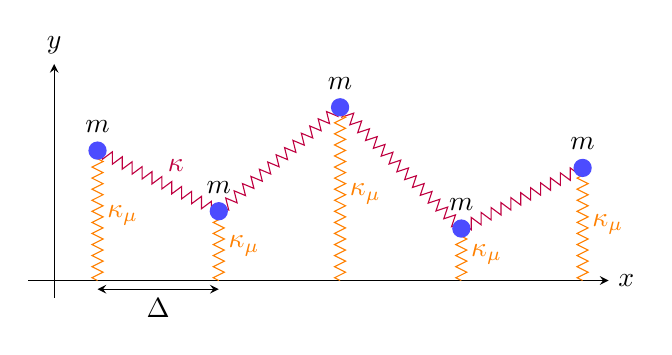
\begin{tikzpicture}[scale=1.1,>=stealth]

            % Horizontal spacing between masses
            \def\Deltax{1.4}

            % Random vertical positions (displacements)
            \def\yA{0.5}
            \def\yB{-0.2}
            \def\yC{1.0}
            \def\yD{-0.4}
            \def\yE{0.3}

            % Reference axes
            \draw[->] (-0.5,-1.2) -- (-0.5,1.5) node[anchor=south]{$y$};
            \draw[->] (-0.8,-1.0) -- (5*\Deltax-1.1,-1.0) node[anchor=west]{$x$};

            % Mass vertical positions
            \coordinate (m1) at (0,\yA);
            \coordinate (m2) at (\Deltax,\yB);
            \coordinate (m3) at (2*\Deltax,\yC);
            \coordinate (m4) at (3*\Deltax,\yD);
            \coordinate (m5) at (4*\Deltax,\yE);

            % Springs (zigzag lines connecting masses)
            \draw[decorate,decoration={zigzag,segment length=4pt,amplitude=2pt}, draw=purple] (m1) -- (m2) node[midway,above right,purple] {$\kappa$};
            \draw[decorate,decoration={zigzag,segment length=4pt,amplitude=2pt}, draw=purple] (m2) -- (m3);
            \draw[decorate,decoration={zigzag,segment length=4pt,amplitude=2pt}, draw=purple] (m3) -- (m4);
            \draw[decorate,decoration={zigzag,segment length=4pt,amplitude=2pt}, draw=purple] (m4) -- (m5);

            % Additional springs for mass term
            \foreach \i/\y in {1/\yA, 2/\yB, 3/\yC, 4/\yD, 5/\yE} {
                    \draw[decorate,decoration={zigzag,segment length=4pt,amplitude=2pt}, draw=orange] (\i*\Deltax-\Deltax,-1) -- (\i*\Deltax-\Deltax,\y) node[midway,right,orange] {$\kappa_{\mu}$};
                }

            % Distance between masses
            \draw[<->] (0,-1.1) -- (\Deltax,-1.1) node[midway,below] {$\Delta$};

            % Masses (blue circles)
            \foreach \m in {m1,m2,m3,m4,m5}{
                    \fill[blue!70] (\m) circle (3pt);
                    \node[above,yshift=3pt] at (\m) {$m$};
                }

        \end{tikzpicture}
    \end{minipage}
    \hfill
    \begin{minipage}{0.45\textwidth}
        The additional elastic constant \(\kappa_\mu\) that tends to restore each particle to its equilibrium position is directly related to the inertial mass of the corresponding particle field.

        For the discrete chain, the Lagrangian can be written as:
    \end{minipage}
\end{figure}
\[
    L = \sum_{j=1}^N \left[ \frac{1}{2} m \dot{y}_j^2  - \frac{1}{2} m v^2 \left( \frac{y_j - y_{j+1}}{\Delta} \right)^2 - \frac{1}{2} \kappa_\mu y_j^2 \right].
\]

Passing to the continuum limit, the discrete sums and differences are replaced by integrals and derivatives:
\[
    \begin{aligned}
        \sum_{j=1}^N                                  & \longrightarrow \int \dd x,                                             \\
        y_j^2                                         & \longrightarrow \psi(x,t)^2,                                            \\
        \dot{y}_j^2                                   & \longrightarrow \left( \frac{\partial \psi(x,t)}{\partial t} \right)^2, \\
        \left( \frac{y_j - y_{j+1}}{\Delta} \right)^2 & \longrightarrow \left( \frac{\partial \psi(x,t)}{\partial x} \right)^2.
    \end{aligned}
\]

Thus, the continuum Lagrangian (with \(v=c=1\)) reads:
\[
    L = \frac{1}{2}m \int \dd x \left[ \left( \frac{\partial \psi(x,t)}{\partial t} \right)^2 - \left( \frac{\partial \psi(x,t)}{\partial x} \right)^2 - \frac{\kappa_\mu}{m} \psi(x,t)^2 \right],
\]
where the last term plays the role of a mass term, proportional to \(m^2\) in natural units. This formulation makes clear how a restoring interaction at the discrete level leads, in the continuum limit, to a massive field with excitations corresponding to massive particles.

Let us now introduce the \textbf{Lagrangian density} \(\mathcal{L}\), which allows us to describe the system in the continuum and relativistic framework. The total Lagrangian is obtained by integrating the Lagrangian density over all space:
\[
    L = \int_{-\infty}^{\infty} \d{x} \mathcal{L}, \quad \text{so that the action reads} \quad S = \int \d{t} L = \int \d{t} \d{x} \mathcal{L}.
\]
Here we integrate along the entire real axis, reflecting the fact that we consider the chain to be infinitely long in the continuum limit.

For the discrete Lagrangian derived previously, the corresponding density is:
\[
    \mathcal{L} = \frac{m}{2} \left[ (\partial_t \psi)^2 - (\partial_x \psi)^2 \right] - \frac{\kappa_\mu}{2} \psi^2.
\]

\paragraph{Minkowski metric and derivatives}
To make contact with special relativity, we need to account for the Minkowski metric, using the \textit{mostly-minus} convention to ensure the correct sign of the kinetic term:
\[
    \eta_{\mu \nu} = \begin{pmatrix}
        1 & 0  & 0  & 0  \\
        0 & -1 & 0  & 0  \\
        0 & 0  & -1 & 0  \\
        0 & 0  & 0  & -1
    \end{pmatrix} = \eta^{\mu \nu}, \quad \mu,\nu = 0,1,2,3.
\]
In our 1-dimensional spatial model, the derivatives transform as:
\[
    \partial_\mu = \frac{\partial}{\partial x^\mu} = \eta_{\mu \nu} \partial^\nu = \eta_{\mu \nu} \frac{\partial}{\partial x_\nu},
    \quad \text{so that} \quad
    \partial_0 = \frac{\partial}{\partial t} = \partial^0,
    \quad
    \partial_1 = \frac{\partial}{\partial x} = - \partial^1.
\]

With this convention, the Minkowski contraction of derivatives reads:
\[
    \partial_\mu \psi \, \partial^\mu \psi = \eta^{\mu \nu} \partial_\mu \psi \, \partial_\nu \psi = (\partial_0 \psi)^2 - (\partial_1 \psi)^2 = (\partial_t \psi)^2 - (\partial_x \psi)^2.
\]

\paragraph{Relativistic form of the Lagrangian density}

Finally, we can express the Lagrangian density in a manifestly Lorentz-covariant form:
\[
    \mathcal{L} = \frac{m}{2} \, \partial_\mu \psi \, \partial^\mu \psi - \frac{\kappa_\mu}{2} \psi^2,
\]
where the second term plays the role of a mass term, endowing the field \(\psi\) with an effective rest energy proportional to \(m^2\). This compact form makes the relativistic structure of the theory explicit and allows for a straightforward generalization to higher-dimensional field theories. Moreover, it provides a natural route to the corresponding equations of motion through the Euler–Lagrange formalism in relativistic notation.

Let us now derive the field equations explicitly. The Euler–Lagrange equations for a continuous field \(\psi(x,t)\) read:
\[
    \frac{\partial}{\partial t} \frac{\partial \mathcal{L}}{\partial (\partial_t \psi)}
    = \frac{\partial \mathcal{L}}{\partial \psi}
    - \frac{\partial}{\partial x} \frac{\partial \mathcal{L}}{\partial (\partial_x \psi)}.
\]
Here, the spatial derivative term arises from the elastic contribution associated with the stiffness constant \(\kappa_\mu\). Computing these derivatives gives:
\[
    m \, \frac{\partial^2 \psi(x,t)}{\partial t^2}
    = m \, \frac{\partial^2 \psi(x,t)}{\partial x^2} - \kappa_\mu \psi(x,t),
\]
which can be rearranged as
\[
    \partial_t^2 \psi - \partial_x^2 \psi = -\frac{\kappa_\mu}{m} \, \psi.
\]
Introducing the \textit{D’Alembert operator} (or box operator)
\[
    \Box = \eta^{\mu\nu}\partial_\mu \partial_\nu = \partial_t^2 - \partial_x^2,
\]
the field equation takes the compact relativistic form
\[
    \left( \Box + \frac{\kappa_\mu}{m} \right) \psi(x,t) = 0.
\]

To analyze the dynamics more conveniently, we perform a Fourier transform that diagonalizes the spatial dependence:
\[
    \psi(x,t) = \frac{1}{2\pi} \int_{-\infty}^{+\infty} \! d\kappa \, e^{i\kappa x} \, \tilde{\psi}(\kappa,t),
\]
which represents the continuum limit of the discrete Fourier series
\[
    y_j(t) = \frac{1}{\sqrt{N}} \sum_{\sigma=1}^{N} e^{i\kappa_\sigma (\Delta j)} \tilde{y}_\sigma(t),
    \qquad
    \kappa_\sigma = \frac{2\pi}{\Delta N}\sigma,
    \qquad
    (\Delta j) = x.
\]
As in the discrete case, we require the field \(\psi(x,t)\) to be real, implying that
\[
    \tilde{\psi}(\kappa,t) = \tilde{\psi}^*(\kappa,t) = \tilde{\psi}(-\kappa,t).
\]
Differentiating under the integral sign, we obtain
\[
    \begin{aligned}
        \partial_t^2 \psi(x,t) & = \frac{1}{2\pi} \int_{-\infty}^{+\infty} d\kappa \, e^{i \kappa x} \, \ddot{\tilde{\psi}}(\kappa,t),         \\
        \partial_x^2 \psi(x,t) & = \frac{1}{2\pi} \int_{-\infty}^{+\infty} d\kappa \, (-\kappa^2) \, e^{i \kappa x} \, \tilde{\psi}(\kappa,t),
    \end{aligned}
\]
which leads to the following evolution equation for each Fourier mode:
\[
    \ddot{\tilde{\psi}}(\kappa,t) = -\left( \kappa^2 + \frac{\kappa_\mu}{m} \right) \tilde{\psi}(\kappa,t).
\]
This is the equation of motion of a harmonic oscillator with frequency
\[
    \omega_\kappa = \sqrt{\kappa^2 + \frac{\kappa_\mu}{m}},
\]
so that in momentum space we have
\[
    \ddot{\tilde{\psi}}(\kappa,t) + \omega_\kappa^2 \tilde{\psi}(\kappa,t) = 0.
\]

\begin{figure}[H]
    \begin{minipage}{0.6\textwidth}
        \centering
        \begin{tikzpicture}
            \begin{axis}[
                    axis lines=middle,
                    xlabel={$\kappa$},
                    ylabel={$\omega_{\kappa}$},
                    grid=none,
                    domain=-3:3,
                    samples=200,
                    ymin=-0.2, ymax=4,
                    xtick=\empty,
                    ytick=\empty,
                    width=8cm,
                    height=5cm,
                    title={$\omega_{\kappa} = \sqrt{\kappa^2 + \mu^2}$ with $\mu=\sqrt{\tfrac{\kappa_\mu}{m}}$},
                ]
                \addplot[thick, blue!70] {sqrt(x^2 + 1^2)};
                \addplot[dashed, gray] coordinates {(1,0) (1,1.4)};
                \addplot[dashed, gray] coordinates {(-1,0) (-1,1.4)};
                \node[anchor=west,orange] at (axis cs:0,1.2) {$\mu$};
                \fill[orange] (0,1) circle (2pt);
                \node[anchor=south west,purple] at (axis cs:1,0) {$\overline{\kappa} $};
                \node[anchor=south west,purple] at (axis cs:-1,0) {$-\overline{\kappa} $};
                \fill[purple] (1,0) circle (2pt);
                \fill[purple] (-1,0) circle (2pt);
            \end{axis}
        \end{tikzpicture}
    \end{minipage}
    \hfill
    \begin{minipage}{0.35\textwidth}
        The field $\psi(x,t)$ is real because its Fourier transform satisfies
        $\tilde{\psi}(\kappa,t)=\tilde{\psi}^*(\kappa,t)=\tilde{\psi}(-\kappa,t)$,
        a direct consequence of the symmetry of $\omega_\kappa$ under $\kappa\to-\kappa$.

        The parameter $\kappa_\mu$ sets the particle mass $\mu$, while $m$ may be absorbed in a redefinition of the field or set to unity in natural units.
    \end{minipage}
\end{figure}

We have thus described a system equivalent to an infinite collection of \emph{decoupled harmonic oscillators}, each characterized by its own wavenumber \(\kappa\) and frequency \(\omega_\kappa\):
\[
    \begin{aligned}
        \omega_\kappa^2         & = \kappa^2 + \frac{\kappa_\mu}{m},                 \\
        \hbar^2 \omega_\kappa^2 & = \hbar^2 \kappa^2 + \hbar^2 \frac{\kappa_\mu}{m}, \\
        E^2                     & = p^2 + \mu^2.
    \end{aligned}
\]
Hence, the quanta of excitation of the field obey the relativistic \textit{energy–momentum relation}, identifying \(\mu\) as the particle’s rest mass, determined by
\[
    \kappa_\mu = \frac{\mu^2 m}{\hbar^2}.
\]

Returning to position space, we recover the celebrated \textbf{Klein–Gordon equation} in natural units:
\[
    \left( \Box + \mu^2 \right) \psi(x,t) = 0,
\]
which describes the classical dynamics of a scalar (spin-0) field of mass \(\mu\). Upon quantization, each mode \(\tilde{\psi}(\kappa,t)\) corresponds to a relativistic particle satisfying the previously derived dispersion relation.

The associated Lagrangian densities can now be written both in configuration and in momentum space:
\[
    \mathcal{L}(x,t) = \frac{1}{2} \partial_\mu \psi(x,t) \, \partial^{\mu} \psi(x,t) - \frac{1}{2} \mu^2 \psi^2,
    \qquad
    L = \int dx \, \mathcal{L},
\]
and
\[
    \mathcal{L}(\kappa,t) = \frac{1}{2}\left( \dot{\tilde{\psi}}^2(\kappa,t) - \omega_\kappa^2 \tilde{\psi}^2(\kappa,t) \right),
    \qquad
    L = \int d\kappa \, \mathcal{L}.
\]

\begin{remark}
    This correspondence between a relativistic scalar field and a continuous set of harmonic oscillators is the cornerstone of quantum field theory: quantizing each mode \(\tilde{\psi}(\kappa,t)\) gives rise to particle excitations, while Lorentz invariance ensures that all inertial observers describe the same energy–momentum relation.
\end{remark}

\subsubsection{Quantization}

In order to quantize the field, we promote each of the infinitely many decoupled harmonic oscillators to operators acting on a \textit{Fock space}. This space can be written as the direct sum of Hilbert spaces corresponding to states with a definite number of particles:
\[
    \mathcal{F} = \mathcal{H}_1 \oplus \mathcal{H}_2 \oplus \dots,
\]
where $\mathcal{H}_n$ denotes the Hilbert space of $n$-particle states.

In this framework, the mode amplitudes become operators satisfying canonical commutation relations, and can be expressed as
\[
    \tilde{\psi}_\kappa = \frac{1}{\sqrt{2 \omega_{\kappa}}}
    \left( \hat{a}_{\kappa} + \hat{a}^\dagger_{\kappa} \right),
    \qquad
    \tilde{\pi}_\kappa = -i \sqrt{\frac{\omega_{\kappa}}{2}}
    \left( \hat{a}_{\kappa} - \hat{a}^\dagger_{\kappa} \right),
\]
where $\hat{a}_{\kappa}$ and $\hat{a}^\dagger_{\kappa}$ are, respectively, the annihilation and creation operators for the mode labeled by $\kappa$.

A generic state of the Fock space can then be written as
\[
    (\hat a_{\kappa_1}^\dagger)^{n_1}
    (\hat a_{\kappa_2}^\dagger)^{n_2}
    \dots
    (\hat a_{\kappa_l}^\dagger)^{n_l} \ket{0},
    \qquad
    \text{with } n_1 + n_2 + \dots + n_l = n,
\]
which represents a state with $n_1$ particles of momentum $\kappa_1$, $n_2$ particles of momentum $\kappa_2$, and so on. Each state has a definite energy given by
\[
    E = \sum_{i=1}^l n_i \, \omega_{\kappa_i}
    + \frac{1}{2} \int \! \d{\kappa}\, \omega_{\kappa}.
\]
The first term represents the sum of the energies of all excitations, while the second term is the \textbf{vacuum energy}, i.e.\ the sum of the zero-point energies $\tfrac{1}{2}\omega_{\kappa}$ of all the modes.

To compute the probability of finding the system in a particular Fock state with occupation numbers $(n_1,\dots,n_l)$, one takes the modulus squared of the projection of the wave function onto that state:
\[
    \left|
    \bra{\Psi}
    (\hat a_{\kappa_1}^\dagger)^{n_1}
    (\hat a_{\kappa_2}^\dagger)^{n_2}
    \dots
    (\hat a_{\kappa_l}^\dagger)^{n_l}
    \ket{0}
    \right|^2.
\]
The number operator $\hat{N}_{\kappa} = \hat a_{\kappa}^\dagger \hat a_{\kappa}$ acts on these states as
\[
    \hat{N}_{\kappa_i}
    \Big[
        (\hat a_{\kappa_1}^\dagger)^{n_1}
        (\hat a_{\kappa_2}^\dagger)^{n_2}
        \dots
        (\hat a_{\kappa_l}^\dagger)^{n_l}
        \ket{0}
        \Big]
    = n_i
    \Big[
        (\hat a_{\kappa_1}^\dagger)^{n_1}
        (\hat a_{\kappa_2}^\dagger)^{n_2}
        \dots
        (\hat a_{\kappa_l}^\dagger)^{n_l}
        \ket{0}
        \Big],
\]
thus counting the number of excitations in the mode of frequency $\omega_{\kappa_i}$.

The Hamiltonian of the quantized field can then be written as
\[
    \hat{\mathcal{H}}
    = \int \! \d{\kappa}\, \omega_{\kappa}
    \left( \hat a_{\kappa}^\dagger \hat a_{\kappa} + \frac{1}{2} \right)
    = \int \! \d{\kappa}\, \omega_{\kappa}
    \left( \hat N_{\kappa} + \frac{1}{2} \right),
\]
showing that the total energy is the sum of the energies of $N$ independent, non-interacting excitations.

However, the vacuum energy term diverges:
\[
    E_0 = \frac{1}{2} \int \! \d{\kappa}\, \omega_{\kappa}
    = \frac{1}{2} \int \! \d{\kappa}\, \sqrt{\kappa^2 + \mu^2}.
\]
This divergence is of ultraviolet nature, since it originates from the contribution of arbitrarily high-frequency modes (the continuum limit $\Delta \to 0$). In practice, this means that the theory cannot be valid at all length scales, and that our idealization breaks down beyond a certain energy cutoff.

In the absence of gravity — which would couple directly to the absolute energy density of the vacuum — this infinite constant can be safely neglected, as only energy \emph{differences} have physical meaning in non-gravitational systems. We can therefore redefine the energy scale by setting $E_0 = 0$.

If we introduce a finite cutoff, e.g.\ imposing $\kappa \Delta \leq 1$ for a small but finite $\Delta$, the vacuum energy becomes finite, representing the physically meaningful contribution of modes below that cutoff.

\begin{remark}
    Different Fock states can correspond to the same total energy, since what matters is the combination of occupation numbers and mode frequencies. In this free-field framework, interactions are absent, so transitions between different states cannot occur. Nevertheless, the formalism provides a powerful description of systems with variable particle number: it allows us to represent, for instance, both the initial and final states of a decay or scattering process, even though their microscopic interaction dynamics lie beyond the scope of the free theory. Including interactions would require additional, non-linear terms in the Lagrangian density — corresponding to higher-order terms in its Taylor expansion around the equilibrium (vacuum) configuration.
\end{remark}